% Options for packages loaded elsewhere
\PassOptionsToPackage{unicode}{hyperref}
\PassOptionsToPackage{hyphens}{url}
\documentclass[
]{ltjsarticle}
\usepackage{xcolor}
\usepackage[margin=20mm]{geometry}
\usepackage{amsmath,amssymb}
\setcounter{secnumdepth}{-\maxdimen} % remove section numbering
\usepackage{iftex}
\ifPDFTeX
  \usepackage[T1]{fontenc}
  \usepackage[utf8]{inputenc}
  \usepackage{textcomp} % provide euro and other symbols
\else % if luatex or xetex
  \usepackage{unicode-math} % this also loads fontspec
  \defaultfontfeatures{Scale=MatchLowercase}
  \defaultfontfeatures[\rmfamily]{Ligatures=TeX,Scale=1}
\fi
\usepackage{lmodern}
\ifPDFTeX\else
  % xetex/luatex font selection
\fi
% Use upquote if available, for straight quotes in verbatim environments
\IfFileExists{upquote.sty}{\usepackage{upquote}}{}
\IfFileExists{microtype.sty}{% use microtype if available
  \usepackage[]{microtype}
  \UseMicrotypeSet[protrusion]{basicmath} % disable protrusion for tt fonts
}{}
\makeatletter
\@ifundefined{KOMAClassName}{% if non-KOMA class
  \IfFileExists{parskip.sty}{%
    \usepackage{parskip}
  }{% else
    \setlength{\parindent}{0pt}
    \setlength{\parskip}{6pt plus 2pt minus 1pt}}
}{% if KOMA class
  \KOMAoptions{parskip=half}}
\makeatother
\usepackage{graphicx}
\makeatletter
\newsavebox\pandoc@box
\newcommand*\pandocbounded[1]{% scales image to fit in text height/width
  \sbox\pandoc@box{#1}%
  \Gscale@div\@tempa{\textheight}{\dimexpr\ht\pandoc@box+\dp\pandoc@box\relax}%
  \Gscale@div\@tempb{\linewidth}{\wd\pandoc@box}%
  \ifdim\@tempb\p@<\@tempa\p@\let\@tempa\@tempb\fi% select the smaller of both
  \ifdim\@tempa\p@<\p@\scalebox{\@tempa}{\usebox\pandoc@box}%
  \else\usebox{\pandoc@box}%
  \fi%
}
% Set default figure placement to htbp
\def\fps@figure{htbp}
\makeatother
\setlength{\emergencystretch}{3em} % prevent overfull lines
\providecommand{\tightlist}{%
  \setlength{\itemsep}{0pt}\setlength{\parskip}{0pt}}
\usepackage{bookmark}
\IfFileExists{xurl.sty}{\usepackage{xurl}}{} % add URL line breaks if available
\urlstyle{same}
\hypersetup{
  hidelinks,
  pdfcreator={LaTeX via pandoc}}

\author{}
\date{}

\begin{document}

\section{論文10：創発ゲージ構造}\label{ux8ad6ux658710ux5275ux767aux30b2ux30fcux30b8ux69cbux9020}

\subsection{接続の運動学的一意性・最初のホロノミー・構造群 SO(4)
の強制・スピン持ち上げ・結合定数の運動学的デフォルト}\label{ux63a5ux7d9aux306eux904bux52d5ux5b66ux7684ux4e00ux610fux6027ux6700ux521dux306eux30dbux30edux30ceux30dfux30fcux69cbux9020ux7fa4-so4-ux306eux5f37ux5236ux30b9ux30d4ux30f3ux6301ux3061ux4e0aux3052ux7d50ux5408ux5b9aux6570ux306eux904bux52d5ux5b66ux7684ux30c7ux30d5ux30a9ux30ebux30c8}

著者: 木原 範昭 (Noriaki Kihara) 所属: WF System Co., Ltd. ORCID:
0009-0004-6753-4020 版: v0.3（v0.2 の内容・結果は不変。論文0.5
の変位記録定義に呼称統一＝帳簿/台帳を
変位記録／保存量／不変量／会計（勘定）に整理） 日付: 2026 年 6 月
DOI（本版）: 10.5281/zenodo.20689961 Concept DOI:
10.5281/zenodo.20640464 ライセンス: CC BY 4.0

\begin{center}\rule{0.5\linewidth}{0.5pt}\end{center}

\subsection{要旨}\label{ux8981ux65e8}

本稿は、逆数双対モデル（論文1--9）の中に、ゲージ理論の運動学的骨格が\textbf{ゲージ原理を一度も仮定せずに}出現することを示す。接近の向きは通常と逆である：保存量の在庫・安定性・観測可能性という別の問いを詰めるたびに、ゲージ理論の部品が副産物として現れた。

主結果は次の通りである。(1)
\textbf{接続の運動学的一意性}：各断片の動径方向は局所時間様軸の指標であり（論文6）、接続はこれを輸送しなければならない。時間軸輸送＋捻れなし最小性の二条件は、位置適応フレームの最小回転接続を一意に選ぶ
--- 動力学的入力は不要であった。(2)
\textbf{最初のホロノミー}：相互直交な三断片配置（三脚）の兄弟三角形ホロノミーは
90°
回転であり、その回転角は方向球面上の測地三角形の面積（八分円＝\(\pi/2\)）に\textbf{厳密一致}する（離散輸送が連続曲率を正確に再現）。曲率量子
\(\pi/2\) は殻・階層に依らず普遍である。第二の厳密ホロノミー
\(\arccos(4/5)\) は Niven
の定理により無限位数であり、ホロノミー群は無限である。(3)
\textbf{構造群の連続化定理}：異形状断片間の輸送が要求する 45° 回転を
\(B_4\) に添加して生成される群の閉包は SO(4)
全体である（3次元結晶学的制限による証明）。\textbf{連続ゲージ群は仮定ではなく帰結である。}
(4)
\textbf{曲率の所在}：系譜リンク上の曲率と静的な横断捻れは記録不能でありゲージである（記録定理からの導出）。曲率は兄弟三角形に集中し、内部ゲージ構造が物理的でありうる場所は遷移イベント（頂点）に局在する。(5)
\textbf{スピン持ち上げ}：半角持ち上げは無矛盾であり、三脚ホロノミーはスピン表現で位数8、全軸平面環配置はベクトル表現で自明・スピン表現で
\(-1\) の最初のループを運ぶ。ねじ持ち上げ（回転と並進の結合）はピッチ
\(1/2\) で一意であり、励起次数 \((-1)^{\Sigma|k|}\)
という新しいゲージ不変 \(Z_2\) を同定する。(6)
\textbf{結合定数の運動学的デフォルト}：Wilson 型重みの径数 \(\beta\)
について、現行公理系の下では純数え上げ（\(\beta=0\)）が強制されることを示す
--- 有限の \(\beta\) は真に新しい動力学的入力を意味する。

最後に、出現したゲージ構造が Yang--Mills
型ではなく\textbf{一階形式の重力（フィアバイン＋スピン接続）型}であることを同定する。本稿の名乗りは「ゲージ構造＋計算されたホロノミー」までであり、「ゲージ理論」を名乗らない。

\begin{center}\rule{0.5\linewidth}{0.5pt}\end{center}

\subsection{キーワード}\label{ux30adux30fcux30efux30fcux30c9}

格子ゲージ理論、接続、ホロノミー、平行移動、超八面体群、結晶学的制限、スピン構造、二重被覆、Wilson
作用、フィアバイン

\begin{center}\rule{0.5\linewidth}{0.5pt}\end{center}

\subsection{1. はじめに}\label{ux306fux3058ux3081ux306b}

格子の上のゲージ理論は Wilson {[}5{]}
以来、連続ゲージ群を離散時空に載せる構成として確立している（概説は Kogut
{[}6{]}）。本稿の構成は向きが逆である：\textbf{離散構造（\(B_4\)
対称な格子と配置統計）が先にあり、連続群が強制される}。また通常のゲージ理論
{[}7{]}
が内部対称性の局所化から出発するのに対し、本稿で出現するのは各断片の正規直交枠の輸送則
--- 重力の一階形式（Cartan
のフレーム形式）に近い対象である。離散幾何で曲率を扱う伝統は Regge
{[}8{]} に遡る。

本稿の問いは控えめである：論文7で構成された多断片配置に、フレームの整列という構造を\textbf{最小の選択で}与えると何が決まり、何が自由に残るか。

\begin{center}\rule{0.5\linewidth}{0.5pt}\end{center}

\subsection{2.
設定：グラフ・フレーム・リンク}\label{ux8a2dux5b9aux30b0ux30e9ux30d5ux30d5ux30ecux30fcux30e0ux30eaux30f3ux30af}

論文4 {[}1{]} の分裂表現に従い、一回の分裂イベント \(9\to(s_A,s_B,s_C)\)
に対し、ノード＝親と子（各自の内部格子の正規直交4枠を持つ）、リンク＝系譜リンクと兄弟リンク、最小閉路＝兄弟三角形とする。子
\(X\) は親格子のセル \(k_X\) を占有する（配置読み、論文7 {[}3{]}）。

フレーム規約の候補は二つある：(L)
全子が親の格子枠を継承（全リンク恒等、全ホロノミー自明）、(A)
子のフレーム第1ベクトル＝自セル方向 \(\hat k_X\)（位置適応）。

\begin{center}\rule{0.5\linewidth}{0.5pt}\end{center}

\subsection{3.
接続の運動学的一意性}\label{ux63a5ux7d9aux306eux904bux52d5ux5b66ux7684ux4e00ux610fux6027}

\subsubsection{3.1
時間軸輸送条件}\label{ux6642ux9593ux8ef8ux8f38ux9001ux6761ux4ef6}

論文6 {[}2{]} により、非対称ビットの階層内での発現は動径方向に集中する
--- 各断片の動径方向 \(\hat k_X\)
はその断片の\textbf{局所時間様軸の指標}である。接続がこの構造と両立するための必要条件は、リンク変数が動径方向を動径方向へ写すこと：\(U_{AB}(\hat k_A)=\hat k_B\)。格子規約
(L) は \(\hat k_A\ne\hat k_B\) のとき A の時間様軸を B
の空間様方向に写し、\(1{+}3\)
分解の階層普遍性と両立しない。\textbf{よって (L) は排除される。}

\subsubsection{3.2 一意性定理}\label{ux4e00ux610fux6027ux5b9aux7406}

時間軸輸送条件の下で残る横断面の捻れに\textbf{捻れなし条件}（2方向の張る平面の直交補空間上で恒等＝最小回転）を課せば：

\begin{quote}
\textbf{定理}:
時間軸輸送＋捻れなしを満たす接続は、位置適応の最小回転接続に一意に一致する。動力学的入力は不要である。
\end{quote}

非対蹠な軸型方向対に対し最小回転は一意の 90° 回転であり、\(B_4\)
の元である。

\begin{center}\rule{0.5\linewidth}{0.5pt}\end{center}

\subsection{4. ホロノミー}\label{ux30dbux30edux30ceux30dfux30fc}

\subsubsection{4.1
最初のホロノミー：三脚は四分の一回転を運ぶ}\label{ux6700ux521dux306eux30dbux30edux30ceux30dfux30fcux4e09ux811aux306fux56dbux5206ux306eux4e00ux56deux8ee2ux3092ux904bux3076}

相互直交配置 \(\{e_1,e_2,e_3\}\)（論文7の三脚クラス）の兄弟三角形
\(e_1\to e_2\to e_3\to e_1\) のホロノミーは

\[
H=(e_2,e_3)\ \text{平面の }90°\text{ 回転（非自明、位数4、}\det=+1\text{）}
\]

である（行列計算は付録）。方向球面上の測地三角形 \((e_1,e_2,e_3)\)
は三直角を持ち面積
\(=\tfrac{3\pi}2-\pi=\tfrac\pi2\)。\textbf{ホロノミー角＝面積}：離散輸送（\(B_4\)
の最小回転）が連続曲率（Gauss--Bonnet）を厳密に再現する。直交三脚の曲率量子
\(\pi/2\) は、方向が相互直交でありさえすれば殻・階層・形状に依らない ---
スケール不変な曲率量子である。

\begin{figure}
\centering
\pandocbounded{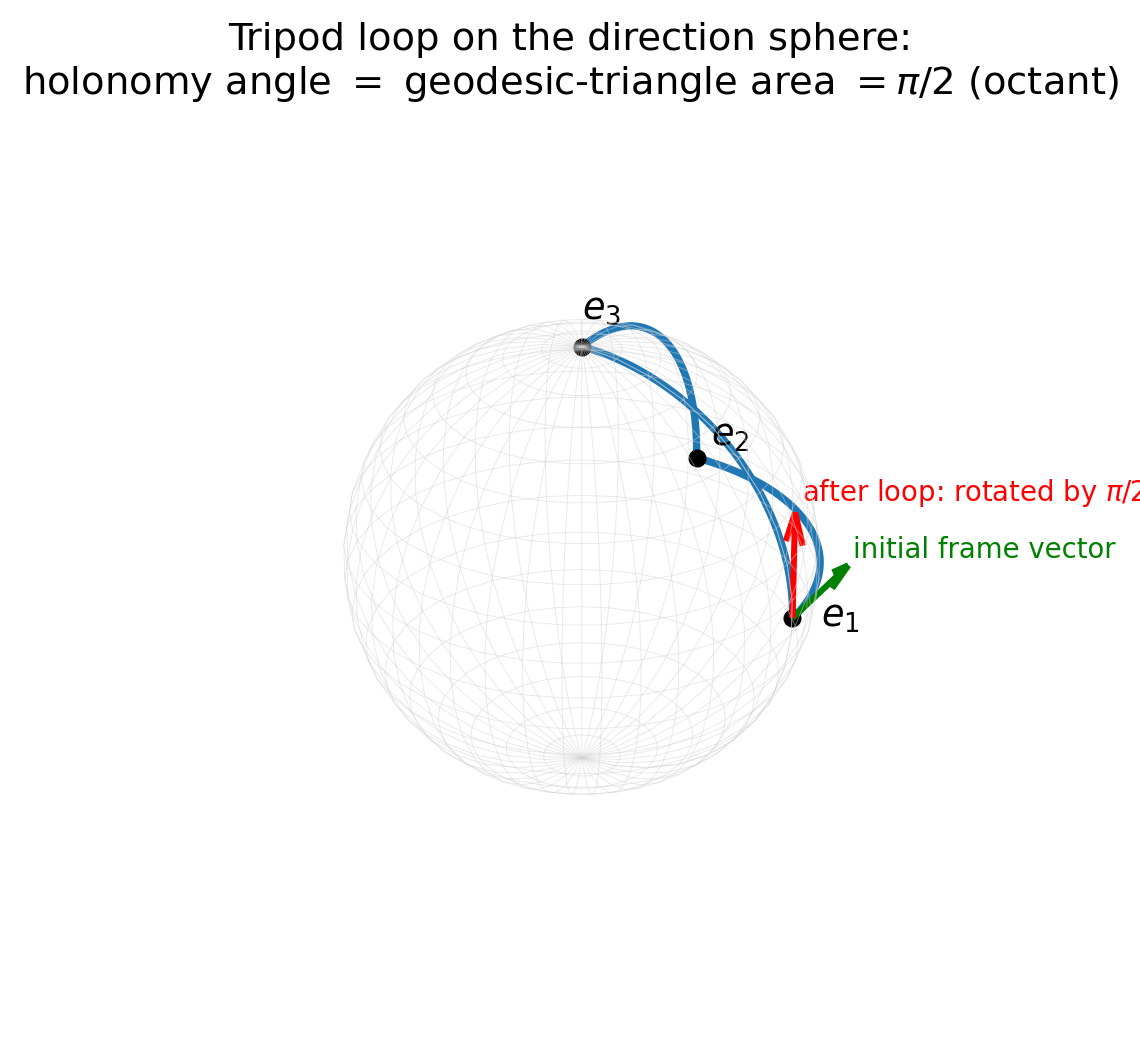
\includegraphics[keepaspectratio,alt={Figure 1. Tripod-loop holonomy equals the geodesic-triangle area}]{figure_paper10_1_tripod_holonomy.png}}
\caption{Figure 1. Tripod-loop holonomy equals the geodesic-triangle
area}
\end{figure}

\textbf{図1.
三脚ループのホロノミー：方向球面上の測地三角形（八分円、三直角）。輸送されたフレームベクトルは一周で
\(\pi/2\) 回転＝三角形面積（Gauss--Bonnet の離散的厳密再現）。}

\subsubsection{4.2
対蹠多義の関係的解消}\label{ux5bfeux8e60ux591aux7fa9ux306eux95a2ux4fc2ux7684ux89e3ux6d88}

対蹠対クラスでは輸送 \(e_1\to-e_1\) が 180°
回転の平面選択を要し一意でない。残る兄弟を経由する測地合成で定義すれば（関係的規則：参照を外部から持ち込まない）、ベクトル表現のホロノミーは正準に自明化する。面積
\(0\) と \(2\pi\)
の差はベクトル表現では不可視であり、スピン持ち上げ（§6）で初めて可視になる。

\subsubsection{4.3
第二の厳密ホロノミーと無限性}\label{ux7b2cux4e8cux306eux53b3ux5bc6ux30dbux30edux30ceux30dfux30fcux3068ux7121ux9650ux6027}

配置 \((2,1,0,0)/\sqrt5,\ (1,2,0,0)/\sqrt5,\ e_3\)
の測地三角形のホロノミー角は球面超過により \(\arccos(4/5)\approx36.87°\)
である。Niven の定理 {[}9{]}（\(\cos\theta\in\mathbb{Q}\) かつ
\(\theta/\pi\in\mathbb{Q}\) なら
\(\cos\theta\in\{0,\pm\tfrac12,\pm1\}\)）により \(\arccos(4/5)/\pi\)
は無理数、よってこのホロノミーは\textbf{無限位数}である。ホロノミー群は無限であり、構造群の連続化（§5）は観測量のレベルで発現する。

\begin{figure}
\centering
\pandocbounded{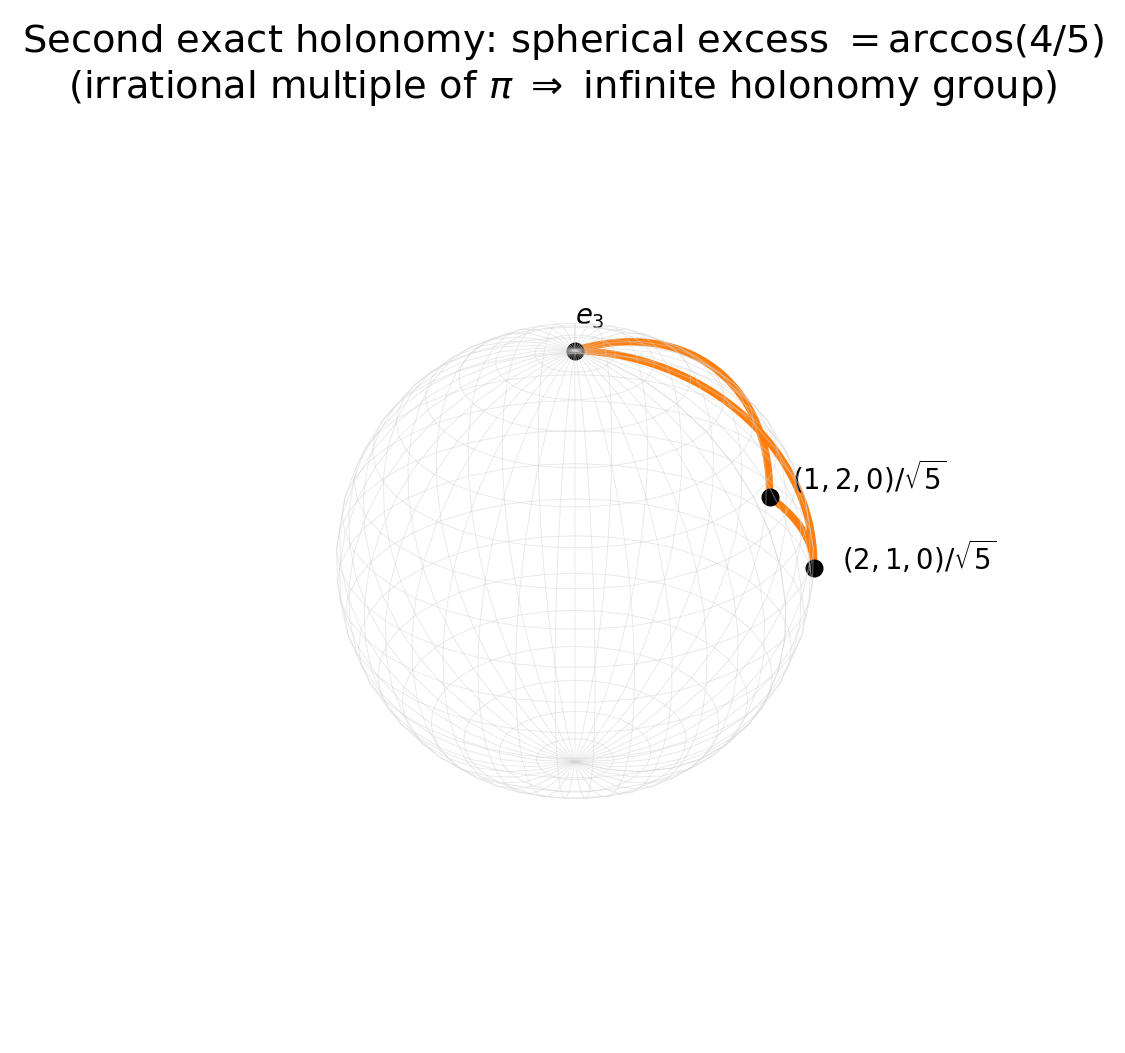
\includegraphics[keepaspectratio,alt={Figure 2. Second exact holonomy: infinite holonomy group}]{figure_paper10_2_holonomy_arccos45.png}}
\caption{Figure 2. Second exact holonomy: infinite holonomy group}
\end{figure}

\textbf{図2. 第二の厳密ホロノミー：配置
\(((2,1,0,0),(1,2,0,0),e_3)/\sqrt5\) 型の球面超過は \(\arccos(4/5)\) ---
\(\pi\) の無理数倍（Niven の定理）であり、ホロノミー群は無限。}

\subsubsection{4.4
曲率の所在（記録定理からの導出）}\label{ux66f2ux7387ux306eux6240ux5728ux8a18ux9332ux5b9aux7406ux304bux3089ux306eux5c0eux51fa}

系譜リンク上に曲率を置いても、その効果が現れるべき従兄弟の相対フレームを読む記録はどの階層にも存在しない（半波長検閲、論文9
{[}4{]}）。記録されない差異には事実がない（記録定理、論文6）から：

\begin{quote}
\textbf{定理}:
系譜曲率と静的な横断捻れはゲージである。曲率の物理的所在は兄弟三角形に限られ（星型平坦は規約ではなく正準ゲージ）、任意の系譜閉路のホロノミーは兄弟三角形ホロノミーの順序積に分解する（離散非可換
Stokes）。内部ゲージ構造が物理的でありうる場所は、リンクではなく\textbf{遷移イベント（頂点）}に局在する。
\end{quote}

\begin{center}\rule{0.5\linewidth}{0.5pt}\end{center}

\subsection{5.
構造群の連続化定理}\label{ux69cbux9020ux7fa4ux306eux9023ux7d9aux5316ux5b9aux7406}

\subsubsection{5.1 障害}\label{ux969cux5bb3}

位置適応では \(U_{AB}(\hat k_A)=\hat k_B\) が必要だが、\(B_4\)（成分
\(\{0,\pm1\}\)）は軸型方向を軸型方向にしか写さない。shell 5
のセル方向は対角型（\((\pm e_i\pm e_j)/\sqrt2\)）であるから、\textbf{異形状間のリンクに
\(B_4\) 値のリンク変数は存在しない}（必要な 45° 回転は成分
\(\pm1/\sqrt2\) を含む）。

\subsubsection{5.2 定理}\label{ux5b9aux7406}

\begin{quote}
\textbf{定理（連続化）}: 異形状リンクが要求する座標平面の 45° 回転を
\(B_4\) に添加して生成される群の閉包は SO(4) 全体である。
\end{quote}

\textbf{証明の骨子}:
二つの相異なる軸まわりの位数8回転を含む3次元有限点群は存在しない（結晶学的制限）。よって生成群は無限であり、その閉包は
SO(3) 部分群族を経て SO(4)
に達する。有限拡大（例：\(W(F_4)\)）でも軌道の長さ別保存により不十分であることを検査済み。∎

\begin{quote}
\textbf{連続ゲージ群は仮定ではなく帰結である。} 目標像は「SO(4)
値接続を持つ離散格子上の構造、その有限 remnant が
\(B_4\)」であり、これは格子ゲージ理論の標準的構図 {[}5,6{]}
と同型である。
\end{quote}

\begin{center}\rule{0.5\linewidth}{0.5pt}\end{center}

\subsection{6.
スピン持ち上げ}\label{ux30b9ux30d4ux30f3ux6301ux3061ux4e0aux3052}

\subsubsection{6.1
構成と無矛盾性}\label{ux69cbux6210ux3068ux7121ux77dbux76feux6027}

各最小回転（角 \(\theta\)）を半角持ち上げ \(\exp(\tfrac\theta2 B)\) で
\(\mathrm{Spin}(4)\)
に持ち上げる。対蹠輸送は関係的規則（§4.2）の合成として持ち上がるため符号が固定され、持ち上げは無矛盾である。四元数計算により三脚ホロノミーの持ち上げは
\(H_{\mathrm{spin}}=(1+i)/\sqrt2\)、\(H_{\mathrm{spin}}^4=-1\)：\textbf{三脚三角形を4周したスピノルは符号反転する}（ベクトル表現では不可視）。

\subsubsection{\texorpdfstring{6.2 最初の
\(-1\)}{6.2 最初の -1}}\label{ux6700ux521dux306e--1}

全軸平面環配置 \(\{e_1,e_2,-e_1,-e_2\}\)
の大円4サイクルはベクトル表現で恒等、スピン表現で \(-1\) ---
\textbf{ベクトル的に自明・スピン的に非自明な最初のループ}である。囲む面積は半球
\(2\pi\)、符号は \((-1)^{\text{面積}/2\pi}\) であり、ループの \(Z_2\)
次数が生まれる。また同種断片の交換の持ち上げは 交換\(^2=-1\)
を与える（スピン統計の素材構造。橋を架けるスピノル的物質は本稿では構成しない）。

\subsubsection{6.3
ねじ持ち上げと励起次数}\label{ux306dux3058ux6301ux3061ux4e0aux3052ux3068ux52b1ux8d77ux6b21ux6570}

現行の実定在波辞書は回転輸送の下で整角（ベクトル的）に変換し、\(-1\)
を検出する物質を含まない（振幅なしの物質は置換表現＝一価、という一般補題による）。半角構造は並進の側にある：実辞書の各セル上でスカラー（±1）として作用する並進は半周期並進のみであり（\textbf{ピッチ
\(1/2\)
の一意性定理}）、回転に並進を結合する\textbf{ねじ持ち上げ}は格子面セクターで一意に定義できる。構造群は直積
\(\mathrm{SO}(4)\times T^4\)（ユークリッド合成では並進が閉路で相殺するため）であり、並進成分は回転に隷属する内部
\(U(1)^4\) 電荷として振る舞う。2π 平面回転のねじ成果はセル \(k\) に
\((-1)^{|k_i|+|k_j|}\) として作用し、新しいゲージ不変次数

\[
\varepsilon(k)=(-1)^{\sum_i|k_i|}
\]

を同定する（殻より細かい：同一殻内に両次数が混在しうる）。なお、2値論理状態・\(Z_2\)
構造・検閲による保護という組合せは、誤り訂正符号と \(Z_2\)
格子ゲージ理論の対応（Kitaev のトーリック符号
{[}10{]}）に構造的に隣接することを記録しておく。ねじ持ち上げの\textbf{導入の必然性}は本稿では未決として明示する。

\begin{figure}
\centering
\pandocbounded{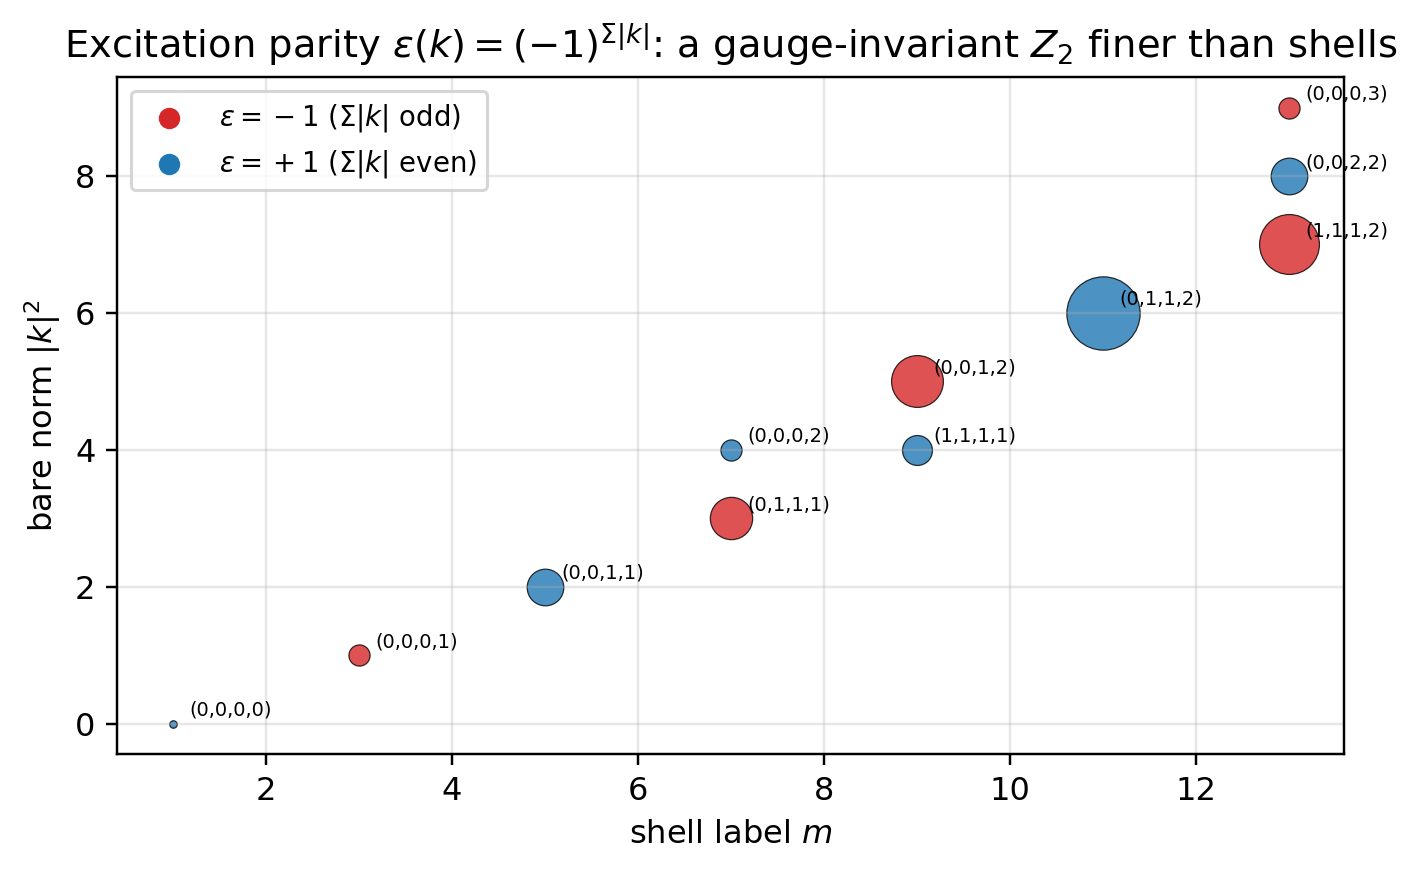
\includegraphics[keepaspectratio,alt={Figure 3. Excitation parity: a gauge-invariant Z2 finer than shells}]{figure_paper10_3_excitation_parity.png}}
\caption{Figure 3. Excitation parity: a gauge-invariant Z2 finer than
shells}
\end{figure}

\textbf{図3. 励起次数 \(\varepsilon(k)=(-1)^{\Sigma|k_i|}\)（\(m\le13\)
全数）：点サイズ＝軌道セル数、色＝パリティ。同一殻内に両次数が混在する
--- 殻より細かいゲージ不変 \(Z_2\)。}

\begin{center}\rule{0.5\linewidth}{0.5pt}\end{center}

\subsection{7.
結合定数の運動学的デフォルト}\label{ux7d50ux5408ux5b9aux6570ux306eux904bux52d5ux5b66ux7684ux30c7ux30d5ux30a9ux30ebux30c8}

兄弟三角形あたり \(s(H)=1-\tfrac14\mathrm{Tr}\,H\)、重み
\(\propto e^{-\beta s}\) の Wilson 型作用 {[}5{]} を考えると、三脚のみが
\(s=\tfrac12\) を担い、分岐比（論文7）は一径数族に変形される。しかし：

\begin{enumerate}
\def\labelenumi{\arabic{enumi}.}
\tightlist
\item
  フレームのフラストレーション（三脚で大域整列が充足不能になること）は、容量・エネルギー・断片内容のすべてで厳密に縮退した配置対（三脚と対蹠対）を分けない
  --- \textbf{面積の会計に借方を立てない}（運動学的に無料）。
\item
  頂点変数（分裂イベントでの子フレーム初期化）の数え上げは、緩和整列で
  \(\beta=0\)、厳密整列で \(\beta=\infty\) の二値しか与えない。
\end{enumerate}

\begin{quote}
\textbf{定理（運動学的デフォルト）}:
現行公理系（三仮定＋配置読み＋記録原理）の下で、分岐比の重みは純数え上げ（\(\beta=0\)）が強制される。有限の
\(\beta\) は真に新しい動力学的入力の存在を意味し、分岐比測定（12.9\% /
0\% /
中間値）が三者判別になる。なお、測度の選択（一括／逐次／経路）が分岐統計に与える差については論文12
§5.3 で扱う。
\end{quote}

\begin{center}\rule{0.5\linewidth}{0.5pt}\end{center}

\subsection{8.
同定と名乗りの規律}\label{ux540cux5b9aux3068ux540dux4e57ux308aux306eux898fux5f8b}

出現した構造の正確な対応相手は、内部対称性の Yang--Mills 理論 {[}7{]}
ではない：位置適応フレーム＝離散的なフレーム場（フィアバイン）、接続＝スピン接続、構造群
SO(4)＝接空間の回転群である。すなわち\textbf{一階形式の重力のゲージ構造}に近い（構造対応であり同一視ではない）。

本稿の名乗りは「ゲージ構造＋計算されたホロノミー」までとする。「ゲージ理論」を名乗るために欠けているもの
--- 伝播するゲージ自由度、作用の動力学、スピノル的物質、内部対称性 ---
は主張範囲の外として明示する。

\begin{center}\rule{0.5\linewidth}{0.5pt}\end{center}

\subsection{9.
本稿の主張範囲}\label{ux672cux7a3fux306eux4e3bux5f35ux7bc4ux56f2}

主張すること：(1) 接続の運動学的一意性（定理）。(2) ホロノミー
\(\pi/2\)＝測地面積（厳密）、\(\arccos(4/5)\)
の無限位数（Niven）、ホロノミー群の無限性。(3) 連続化定理（SO(4)
の強制）。(4)
系譜曲率・静的捻れのゲージ性と曲率の兄弟三角形への集中（記録定理からの導出）。(5)
スピン持ち上げの無矛盾性・位数8・最初の \(-1\)・ピッチ \(1/2\)
の一意性・励起次数 \(\varepsilon\)。(6) \(\beta=0\) の運動学的強制。

主張しないこと：(1) 標準模型のゲージ群・表現・世代構造との対応。(2)
ゲージ場の動力学（伝播・散乱）。(3) フェルミオンの存在（交換\(^2=-1\)
は素材構造であり、スピノル的物質は未構成）。(4)
ねじ持ち上げの必然性。(5) 「ゲージ理論」の名乗り。

\begin{center}\rule{0.5\linewidth}{0.5pt}\end{center}

\subsection{10. 結論}\label{ux7d50ux8ad6}

ゲージ原理を公理に置かずに、接続・曲率・連続構造群・スピン構造・結合定数のデフォルト値までが、安定性と観測可能性の問いの副産物として出現した。とりわけ
(i) 接続が動力学を待たずに運動学で一意に固定されること、(ii)
離散輸送のホロノミーが連続曲率を厳密に再現すること、(iii)
連続群が結晶学的制限によって\textbf{強制}されること、の三点は、離散基礎の上の連続ゲージ構造という構図に対する独立の実例を与える。残る未決
--- 頂点に局在する内部ゲージ場、スピノル的物質、有限結合 ---
は、すべて遷移イベントの構造（頂点写像）という単一の対象に収束している。

\begin{center}\rule{0.5\linewidth}{0.5pt}\end{center}

\subsection{付録：行列と検算}\label{ux4ed8ux9332ux884cux5217ux3068ux691cux7b97}

90° 回転 \(U_{12},U_{23},U_{31}\) の明示行列とホロノミー
\(H=U_{31}U_{23}U_{12}\) の検算（\(e_1\to e_1\), \(e_2\to e_3\),
\(e_3\to-e_2\),
\(H^4=\mathbb1\)）、四元数によるスピン持ち上げ（\(q_3q_2q_1=(1+i)/\sqrt2\)）、障害定理の一行証明（\(B_4\)
成分 \(\{0,\pm1\}\) 対 \(1/\sqrt2\)
の矛盾）、ピッチ一意性の証明（\(2\pi t\in\{0,\pi\}\bmod 2\pi\)）を含む。すべて手計算の厳密代数であり、スクリプトと研究ノートは公開リポジトリ（https://github.com/WurabeSeiji/ai-chat-logs-open）で提供する。

\begin{center}\rule{0.5\linewidth}{0.5pt}\end{center}

\subsection{参考文献}\label{ux53c2ux8003ux6587ux732e}

{[}1{]} 木原 範昭, 論文4, v1.0, 2026. Concept DOI:
10.5281/zenodo.20638962.

{[}2{]} 木原 範昭, 論文6, v0.2, 2026. Concept DOI:
10.5281/zenodo.20640456.

{[}3{]} 木原 範昭, 論文7, v0.2, 2026. Concept DOI:
10.5281/zenodo.20640458.

{[}4{]} 木原 範昭, 論文9, v0.2, 2026. Concept DOI:
10.5281/zenodo.20640462.

{[}5{]} K. G. Wilson, ``Confinement of quarks,'' Physical Review D 10
(1974), 2445--2459.

{[}6{]} J. B. Kogut, ``An introduction to lattice gauge theory and spin
systems,'' Reviews of Modern Physics 51 (1979), 659--713.

{[}7{]} C. N. Yang and R. L. Mills, ``Conservation of isotopic spin and
isotopic gauge invariance,'' Physical Review 96 (1954), 191--195.

{[}8{]} T. Regge, ``General relativity without coordinates,'' Il Nuovo
Cimento 19 (1961), 558--571.

{[}9{]} I. Niven, \emph{Irrational Numbers}, Mathematical Association of
America, 1956.

{[}10{]} A. Kitaev, ``Fault-tolerant quantum computation by anyons,''
Annals of Physics 303 (2003), 2--30.

\begin{center}\rule{0.5\linewidth}{0.5pt}\end{center}

\subsection{ライセンス}\label{ux30e9ux30a4ux30bbux30f3ux30b9}

本稿は CC BY 4.0
に基づき公開する。再利用、翻案、翻訳、引用を許可する。ただし、著者名、版、公開日、出典を明示すること。

\end{document}
